\chapter{Methods}

\section{State of art}
\subsection{Earlier Work}
In recent years, researchers and analysts focused mainly on gray-scale face image. Others, focused and were built on pattern identification models, possessing information of the model while others used AdaBoost. \cite{ojala2002multiresolution} This was a superb classifier for the purpose of training. When Viola-Jones Detector came, which was a breakthrough in face detection technology and real-time face detection became a possibility. Problems faced by this was problems, but not limited to, such as orientation and the brightness which made it hard to intercept. Resulting in its failure to function in dull and dim light, hence, researchers started looking for an alternative model that could overcome this shortcomings.
\subsection{Past Datasets}
Many datasets used in the past for face detection were basically developed to form an impression of face detection models.\cite{nagrath2021ssdmnv2} Earlier datasets had images that were fetched from supervised surroundings whereas current datasets are constructed by compiling online images like WiderFace for example.\cite{yang2016wider}
These current datasets provide annotation compared to previous ones. To make a better training and testing model a large datasets are needed and that helps makes things easier.

\subsection{Current Face Mask Models}
There is a face mask detection model named SSDMNV2 that has been developed using deep neural network modules from OpenCV and Tensorflow that has a Single Shot Multibox Detector object detection model.\cite{nagrath2021ssdmnv2} 
 A face mask has been created by Bosheng Qin and Dongxiao Li 
Method of identification using the classification network SRCNet and achieved a 98.7 percent precision in the classification of images into three groups, namely "correct Wearing a face mask," "wearing a face mask incorrectly" and "wearing no face mask".\cite{qin2020identifying}

G. Jignesh, Narinder Singh, Sanjay Kumar and Sonali Agarwal have noticed that is is difficult to monitor people manually in the public spaces and in their paper proposes a transfer learning model in order to automatically identify people who are wearing a mask and those who are not. \cite{chowdary2020face}
 Narinder Singh, Sanjay Kumar and Sonali Agarwal in a different paper also argue that YOLO v3 object detection model when compared to some state-of-the-art networks it performed better. \cite{punn2020monitoring}
 
 



\section{Technology review}
\subsection{Datasets}
In the process of conducting this experiment, there are two types of datasets. 
The set of fist image datasets are from kaggle.com. The datasets is made up of two classes, those that are with masks and the others that are without masks.
That is a total of 1412 images belonging to 2 classes in training set and 290 images in testing set.


    \centerline{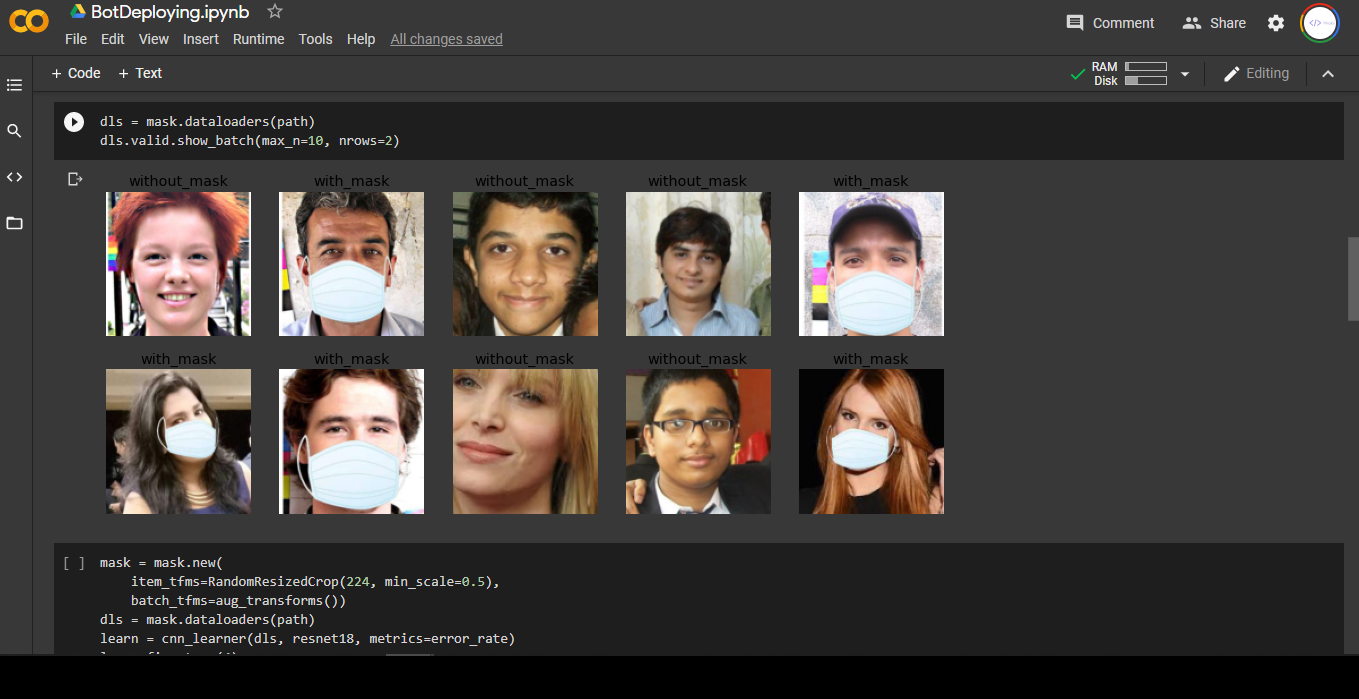
\includegraphics[width=.5\textwidth,height=.5\textheight,keepaspectratio]{tex/images/Screenshot_Masks.png}}
     \caption{Screenshot from my Google Colab}
    \label{fig}

This is what the dataset looks like. We have pictures of people wearing masks and others not wearing masks.  This dataset provides a great variation of faces
this making this dataset useful. To my knowledge this dataset is one of the largest datasets that was released on kaggle that has faces of masks and no masks and made available thanks to Prajna Bhandary.
This dataset was a collection of random faces of people and with the aid of photoshop, some faces were then added masks to make them fit on the face. 
The second set of images are my own collection, where I personally asked people that I know to send me pictures of themselves
with masks, others without so that I can compile a dataset made up of real-world masked faces and capture the different mask colors and shades.

    

\subsection{Convolution Neural Network}
In order to properly tackle Convolutional Neural Network, it is paramount to first understand Machine Learning.
The issue of how to create computers that automatically develop through experience is answered by machine learning. It is one of the fastest growing technical fields today, situated at the intersection between computer science and statistics.\cite{jordan2015machine}
Convolutional Neural Networks have overtaken traditional image recognition methods in the early 2010's. 
Computer vision and image recognition are not the same and must be distinguished. Computer vision is when we allow a computer to imitate or have human-like vision. computer vision means that it can do something. 

image recognition on the other hand is fascinated by pixels and patterns of an image and it recognise an image as it learns more about it.


Convolutional Neural Network comes from Deep Learning or Deep Neural Networks as some would call it and it refers to
Artificial Neural Network with more than one layer. It has gained much attention in the past decade and has been considered as one of the most powerful tools.
Reason for this is its ability to handle enormous amount of data. \cite{albawi2017understanding}

The name is taken from mathematical linear operation between matrixes by the name Convolution. The Convolutional Neural Network
has a good performance on Machine Learning problems, mostly the problems about image data which is why we used it. 




    \centerline{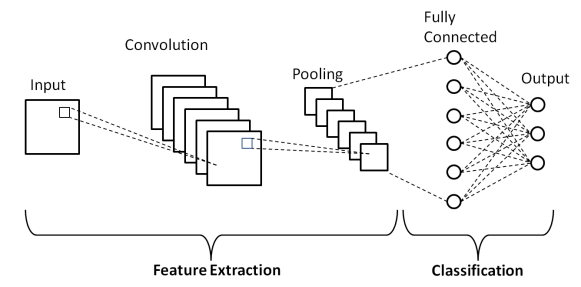
\includegraphics[width=.5\textwidth,height=.7\textheight,keepaspectratio]{tex/images/cnn.jpg}}
    \caption{CNN for fully connected network}
    \label{fig:my_label}
  





The fully connected network is almost similar to how neurons are arranged in a typical neural network.
Each node in a layer is connected directly to every node in both previous and in front layer.

One of the largest limitations of the traditional Neural Network is the fact that they tend to have a hard time 
with computational complexity that is required to process image data, hence the use of CNN becomes vital. \cite{o2015introduction}
As CNNs have become deeper and wider, problems of overfitting have been posed, primarily because of the
Dataset constraints, which are counterproductive to network generalization. For the avoidance of over-fitting,
One way is to alter the design of neural networks by adding dropout layers for example.


\subsection{Transfer Learning}
Transfer learning from a pre-trained network was used.
Transfer learning refers to an improved learning in a new task from a previously trained network. 
Transfer learning is machine learning with an additional source of information
apart from the standard training data: knowledge from one or more related tasks.\cite{torrey2010transfer}

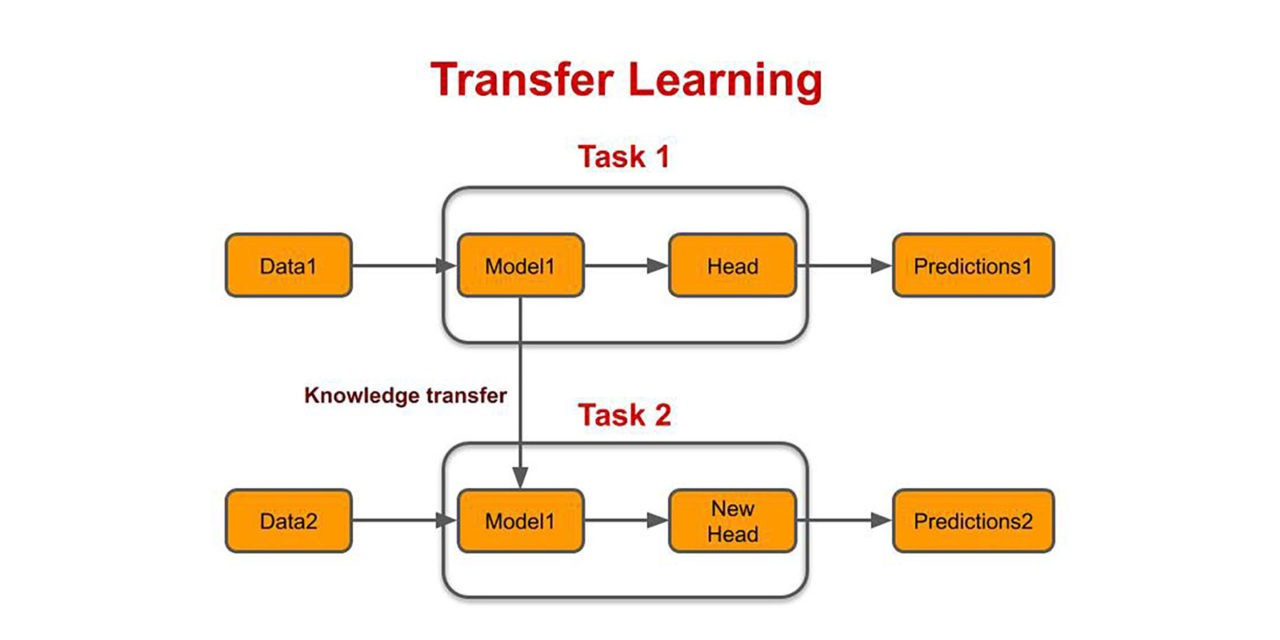
\includegraphics[width=.6\textwidth,height=.7\textheight,keepaspectratio]{tex/images/Transfer.jpeg}
\caption{Transfer Learning Model.}

Thanks to this method, there is no need to re-train the entire model and as a result what is left is to work on the filan classification part.
The InceptionV3 model is an architecture of convolutional networks. It is considered as one of the most accurate models for image classification. It was originally created by the Google Brain team.\cite{hussain2018study}
A transfer learning-based methodology is proposed in this paper that uses the
Pre-trained model for InceptionV3 to identify people who do not wear
Mask for the ears. The last layer of InceptionV3 is removed for this work and is tuned by adding 5 additional layers to the network. 
The 5 added layers are an
A typical pooling layer with a pool size equal to 5 x 5 was followed by a flattening layer,
A dense layer of 128 neurons with the activation and dropout feature of ReLU
A 0.5 rate, and finally a significant dense layer of two neurons and softmax. To classify if a person is wearing a mask, the activation feature is added. Sinno and Qiang \cite{pan2009survey}
in their paper have categorized Tansfer Learning techniques into three:
\begin{itemize}
    \item What transfer,
    \item How to transfer it and
    \item When to transfer it.
\end{itemize}

“What to transfer” asks which part of expertise can
be transferred throughout domain names or tasks. Some expertise is
precise for character domain names or tasks, and a few expertise
can be not unusual place among special domain names such that they may
assist enhance overall performance for the goal area or task. "How to transfer" is a product of which expertise may be transferred, learning
algorithms want to be advanced to switch the expertise. "When to transfer" then address the issue that asks wherein situations, transferring
abilities need to be done. Likewise, we're inquisitive about knowing
wherein situations, understanding need to now no longer be transferred


\subsection{Variational Autoencoder}

 It is a given fact that Deep Learning models has been exceedingly successful at learning data such as images, audio, and so on. However, it also has its limitations
 or challenges. Some of the challenges being biasedness when it comes to various things such as, but not limited to; skin color, gender, angle, etc. 
 Machine learning systems are increasingly making our day-to-day decisions that impact us daily as individual and also as a society. The development of an unbiased AI system
 like the one we have created is of paramount importance to limiting unintended side effects. \cite{amini2019uncovering} 
 Autoencoders are trained to reconstruct the input data. Taking images as an input data in our case.
 Autoencoders are divided into two components, Encoders and Decoders.
 \item Encoder: a number of layers that are fully connected convolutional. They take he input and compress it down to very small representation
 to create what we call a bottleneck. 
 \item Decoded: A reconstruction from the bottleneck that gives the input of fully connected Convolution.
Variational Autoencoders provide a way to debias the image set, removing any bias towards variations in face positions, angle, and race.


A Variational Autoencoder (VAE) is an encoder that has a training that is regularised to avoid over-fitting and ensure that the 
latent space thus has good aspects that allow generative process.  

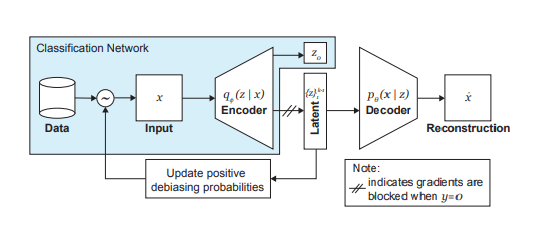
\includegraphics[width=.6\textwidth,height=.7\textheight,keepaspectratio]{tex/images/vae.png}
\caption{Debiasing Variational Autoencoder.}

To minimise the biasedness of our dataset, we train a VAE model to learn the latend structure that takes our dataset and debiases them with respect to facial features.


\subsection{TensorFlow}
A widely used Machine Learning (ML) task program is TensorFlow (TF). It is generally adopted, as it offers an interface to express the models' typical ML algorithms and executable code. Models generated in TensorFlow  can be transported with devices ranging from heterogeneous systems with little to no shift.
From cell phones to servers that are distributed. TensorFlow  has been developed by and is maintained by Google and is used internally within the organization for the purposes of Machine Learning.
In our system, Tensorflow is thus a preferred library that we used.


\subsection{OpenCV}
OpenCV is short for Open Source Computer vision. OpenCV is an open source image and video processing library that was originally introduced by Intel more than a decade ago.  \cite{culjak2012brief}

The basic image processing and higher level computer vision algorithms are contained in the CV component.
We have used an OpenCV for the detection of real-live movement on the web-cam to be able to detect the movement of the face as well as the mask. The use of this library is both easy to use and is relevant in this system. 

In our system we started by importing the CV2 and we use the CV2.VideoCapture to use the camera. Furthermore, we use CascadeClassifier to load the XML file 'haarcascade frontalface default.xml'

cv2.resize is then used to resize the image to speed up the detection. cv2.rectangle are used to draw rectangles across the faces. cv2.show is to go live and display the webcam.




\section{References}

\section{Equations}

